\documentclass[a4paper,11pt]{article}
\usepackage{amsmath,amsthm,amsfonts,amssymb,bm} 
\usepackage{graphicx,psfrag} 
\usepackage{fancyhdr}
\usepackage{color} 
\usepackage{geometry}
\usepackage{multirow}
\usepackage{listings}
\usepackage{enumerate}
\usepackage{leftidx} 
\usepackage{mathrsfs} 

\usepackage{listings}
\usepackage{color}

\definecolor{mygreen}{rgb}{0,0.6,0}
\definecolor{mygray}{rgb}{0.5,0.5,0.5}
\definecolor{mymauve}{rgb}{0.58,0,0.82}

\lstset{ %
  backgroundcolor=\color{white},   % choose the background color; you must add \usepackage{color} or \usepackage{xcolor}
  basicstyle=\footnotesize,        % the size of the fonts that are used for the code
  breakatwhitespace=false,         % sets if automatic breaks should only happen at whitespace
  breaklines=true,                 % sets automatic line breaking
  captionpos=b,                    % sets the caption-position to bottom
  commentstyle=\color{mygreen},    % comment style
  deletekeywords={...},            % if you want to delete keywords from the given language
  escapeinside={\%*}{*)},          % if you want to add LaTeX within your code
  extendedchars=true,              % lets you use non-ASCII characters; for 8-bits encodings only, does not work with UTF-8
  keepspaces=true,                 % keeps spaces in text, useful for keeping indentation of code (possibly needs columns=flexible)
  keywordstyle=\bfseries,       % keyword style
  language=SQL,                 % the language of the code
  morekeywords={*,...},            % if you want to add more keywords to the set
  numbers=none,                    % where to put the line-numbers; possible values are (none, left, right)
  numbersep=5pt,                   % how far the line-numbers are from the code
  numberstyle=\tiny\color{mygray}, % the style that is used for the line-numbers
  rulecolor=\color{black},         % if not set, the frame-color may be changed on line-breaks within not-black text (e.g. comments (green here))
  showspaces=false,                % show spaces everywhere adding particular underscores; it overrides 'showstringspaces'
  showstringspaces=false,          % underline spaces within strings only
  showtabs=false,                  % show tabs within strings adding particular underscores
  stepnumber=2,                    % the step between two line-numbers. If it's 1, each line will be numbered
  stringstyle=\color{mymauve},     % string literal style
  tabsize=2,                       % sets default tabsize to 2 spaces
  title=\lstname                   % show the filename of files included with \lstinputlisting; also try caption instead of title
}

\geometry{left=3.17cm,right=3.17cm,top=2.54cm,bottom=2.54cm}

\begin{document}

\pagestyle{fancy}
\rfoot{\thepage}
\rhead{\bfseries Database System Concept}
\setlength{\parskip}{0.7ex plus0.2ex minus0.2ex}
\cfoot{\empty}
\lhead{\empty}


\title{Assignment 7}
\author{Qinglin Li, 5110309074}
\date{}
\maketitle

\headheight 3pt
\thispagestyle{fancy}
\section*{Problem 1}
\begin{enumerate}[a.]
\item ~\\ 
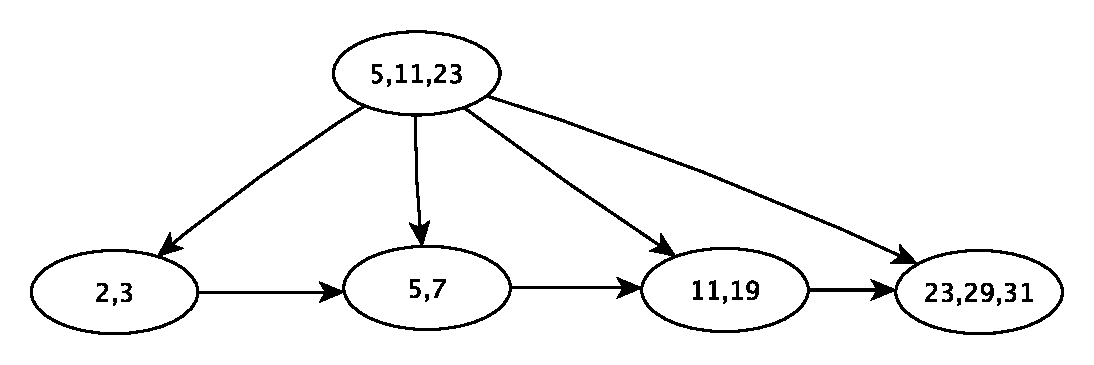
\includegraphics[scale=0.8]{1-1}
\item ~\\
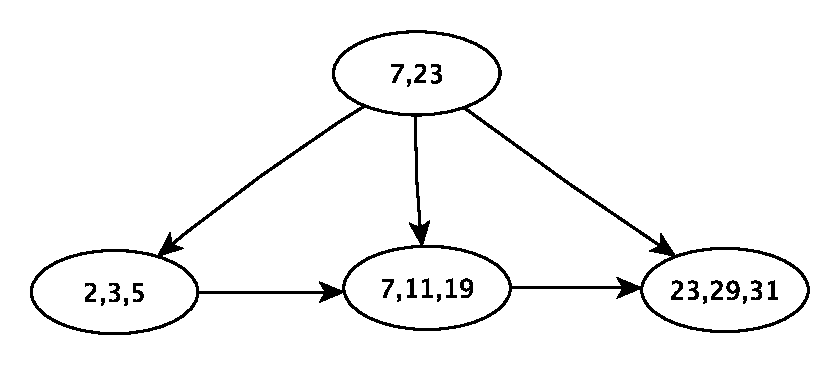
\includegraphics[scale=0.8]{1-2}
\item ~\\
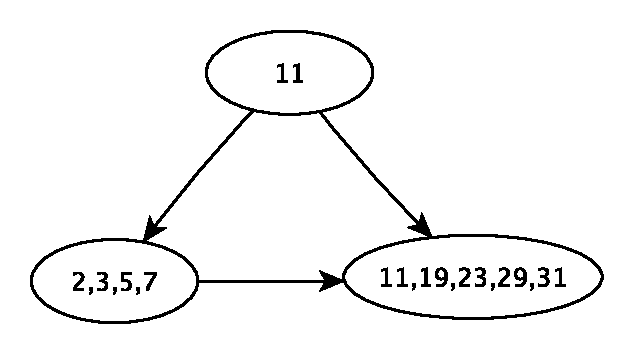
\includegraphics[scale=0.8]{1-3}
\end{enumerate}
\newpage

\section*{Problem 2}
\subsection*{Four pointers}
\begin{enumerate}[a.]
    \item ~\\
        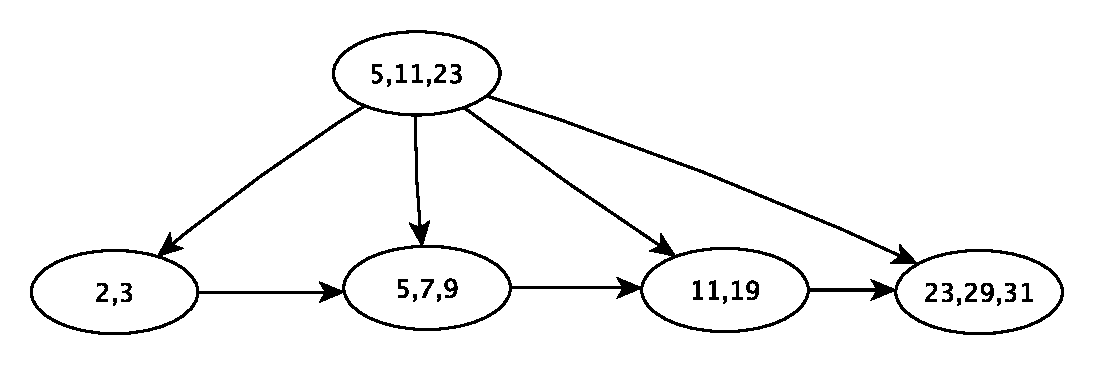
\includegraphics[scale=0.7]{2-1-1}
    \item ~\\
        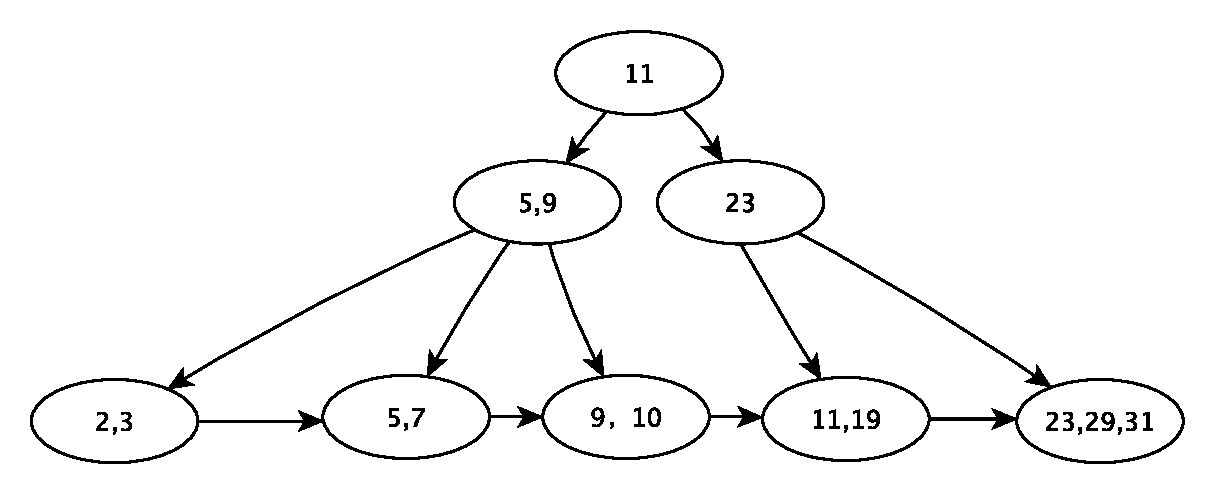
\includegraphics[scale=0.7]{2-1-2}
    \item ~\\
        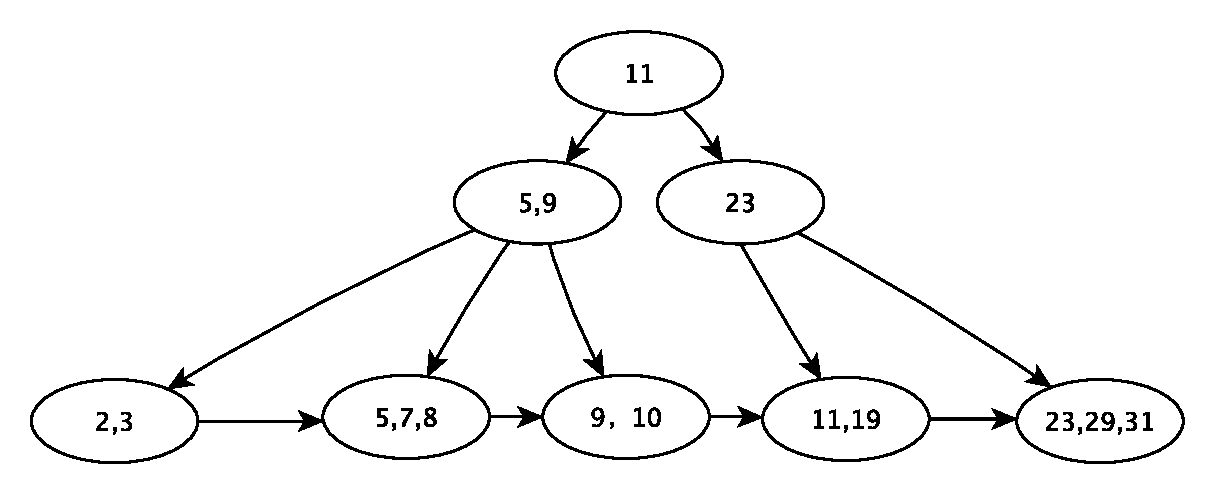
\includegraphics[scale=0.7]{2-1-3}
    \item ~\\
        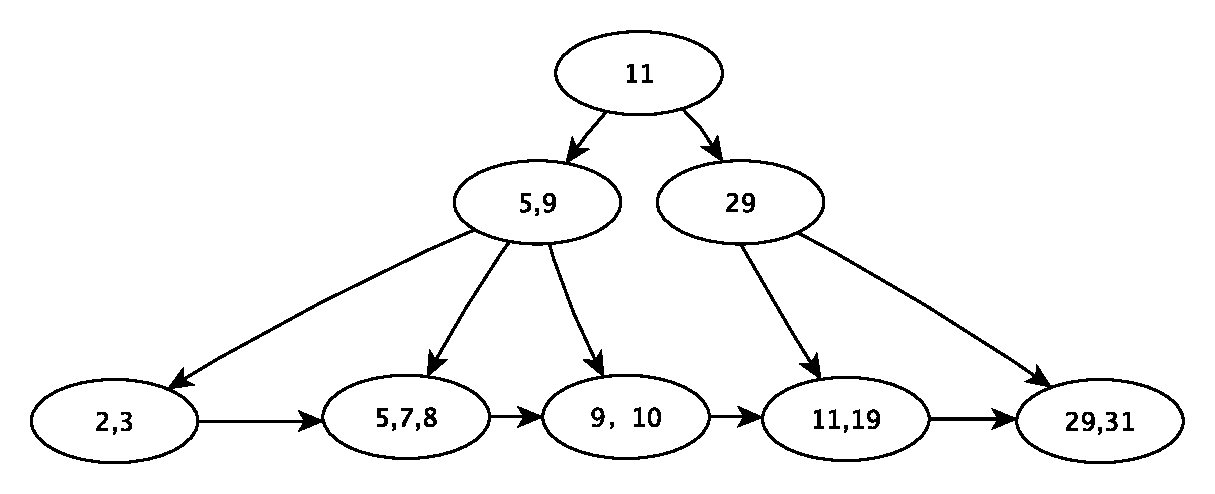
\includegraphics[scale=0.7]{2-1-4}
    \item ~\\
        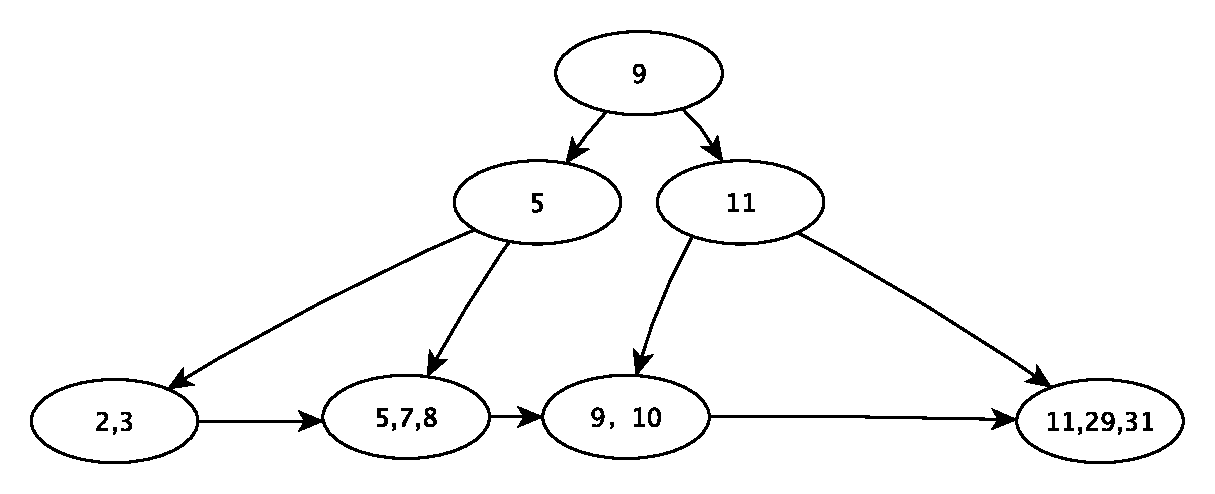
\includegraphics[scale=0.7]{2-1-5}
\end{enumerate}

\subsection*{Six pointers}
\begin{enumerate}[a.]
    \item ~\\
        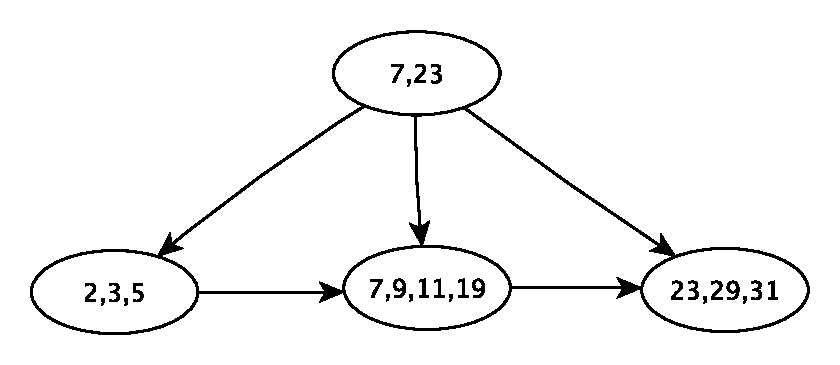
\includegraphics[scale=0.7]{2-2-1}
    \item ~\\
        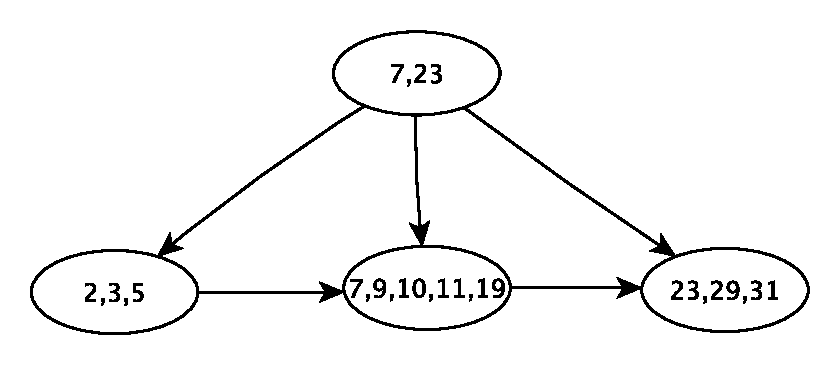
\includegraphics[scale=0.7]{2-2-2}
    \item ~\\
        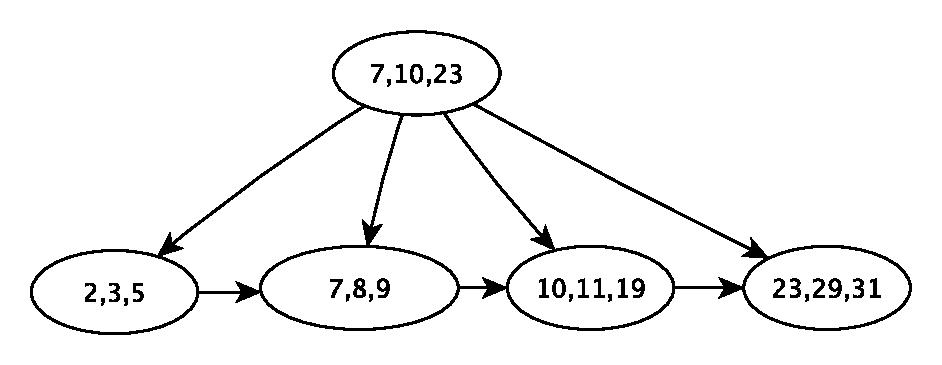
\includegraphics[scale=0.7]{2-2-3}
    \item ~\\
        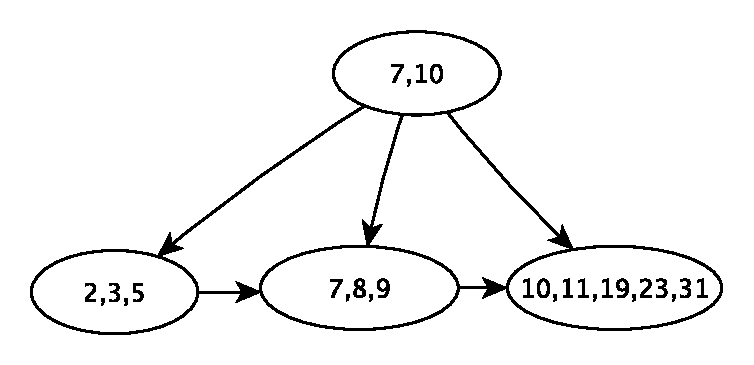
\includegraphics[scale=0.7]{2-2-4}
    \item ~\\
        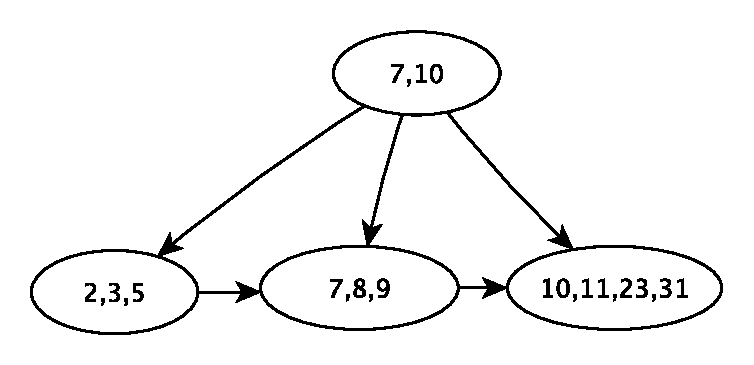
\includegraphics[scale=0.7]{2-2-5}
\end{enumerate}

\subsection*{Eight pointers}
\begin{enumerate}[a.]
    \item ~\\
        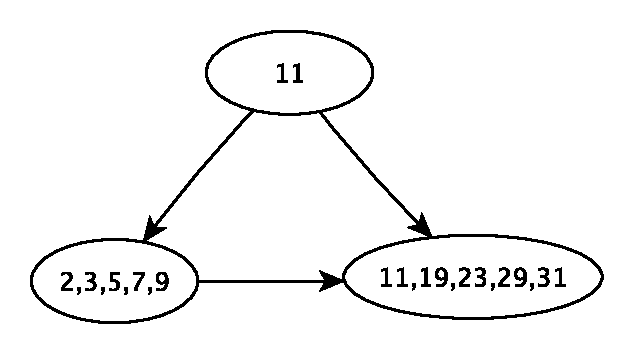
\includegraphics[scale=0.7]{2-3-1}
    \item ~\\
        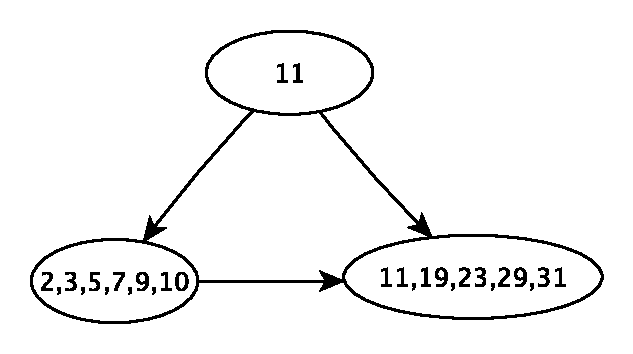
\includegraphics[scale=0.7]{2-3-2}
    \item ~\\
        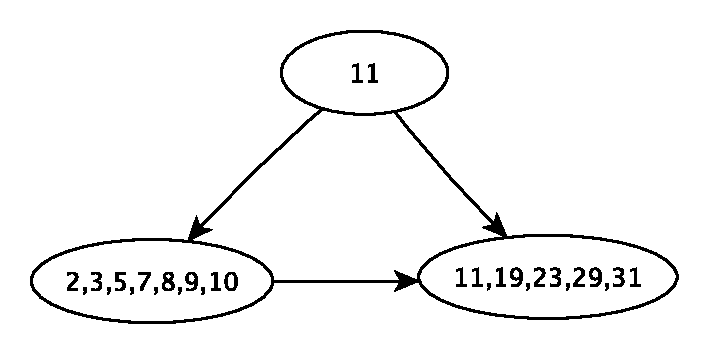
\includegraphics[scale=0.7]{2-3-3}
    \item ~\\
        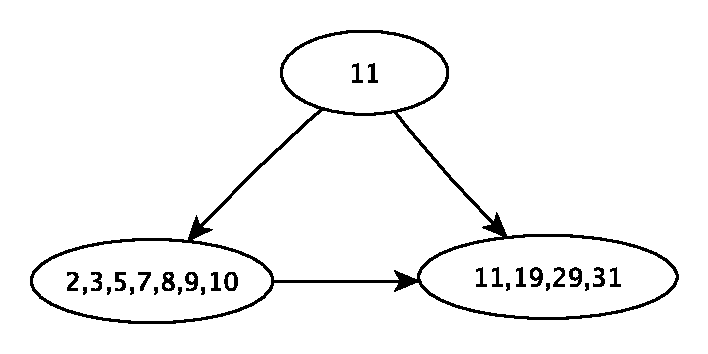
\includegraphics[scale=0.7]{2-3-4}
    \item ~\\
        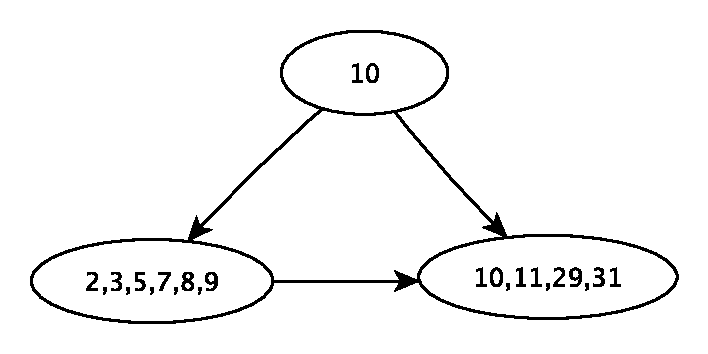
\includegraphics[scale=0.7]{2-3-5}
\end{enumerate}

\section*{Problem 3}
\begin{enumerate}[a.]
\item
Find the first record with $10<A<50$ and enumerate them.\\
So $n_1+h$ times disk I/O is needed.
\item
Since we just need to use the condition $5<B<10$ to test each tuple with $10<A<50$.\\
The cost should be the same as \textbf{a}
\item 
$n_1=n_2$
\end{enumerate}
\section*{Problem 4}
\begin{enumerate}[a.]
\item
Block transfer: $50000\times(45000/30) + 50000/25 = 75002000$\\
Seek: $50000 + 2000=52000$
\item 
Block transfer: $(45000/30)\times(50000/25) + 50000/25 = 3002000$\\
Seek: $2\times(50000/25)=4000$
\item
Since the tuples fit on one block, $\#$Block transfer = $\#$Seek = $(45000/30)+(50000/25)=3500$
\item
Assume the memory is large enough.\\
$\#$Block transfer is approximately $(45000/30+50000/25)\times 3=10500$\\
$\#$Seek: $2\times(50000/25+45000/30)=7000$
\end{enumerate}
\section*{Problem 5}
\begin{enumerate}[a.]
\item
Find the first tuple with $building \geq \text{``Wastson"}$ and use the index to enumerate them.
Union these tuples with tuples having $building = null$.
\item 
Use the techniques as \textbf{a} to find tuples with $building < \text{``Wastson"}$, $building > \text{``Wastson"}$, $building = null$ and union them all.
\item 
Use the techniques as \textbf{a} to find all tuples satisfying $\neg(building < \text{``Wastson"})$.\\
Then union them all and test every tuple with condition $\neg(budget < 50000)$.
\end{enumerate}

\section*{Problem 6}
\begin{enumerate}[a.]
\item
Using pipelining, output from the sorting operation on r is written to a 
buffer $B$. When $B$ is full, the merge-join processes tuples from $B$, 
joining them with tuples from $s$ until $B$ is empty. At this point, the 
sorting operation is resumed and $B$ is refilled. This process continues 
until the merge-join is complete.
\item 
If the sort–merge operations are run in parallel and memory is shared 
equally between the two, each operation will have only $M/2$ frames for 
its memory buffer. This may increase the number of runs required to 
merge the data. 
\end{enumerate}
\end{document}

